\documentclass[12pt,]{book}
\usepackage{lmodern}
\usepackage{amssymb,amsmath}
\usepackage{ifxetex,ifluatex}
\usepackage{fixltx2e} % provides \textsubscript
\ifnum 0\ifxetex 1\fi\ifluatex 1\fi=0 % if pdftex
  \usepackage[T1]{fontenc}
  \usepackage[utf8]{inputenc}
\else % if luatex or xelatex
  \ifxetex
    \usepackage{mathspec}
  \else
    \usepackage{fontspec}
  \fi
  \defaultfontfeatures{Ligatures=TeX,Scale=MatchLowercase}
\fi
% use upquote if available, for straight quotes in verbatim environments
\IfFileExists{upquote.sty}{\usepackage{upquote}}{}
% use microtype if available
\IfFileExists{microtype.sty}{%
\usepackage{microtype}
\UseMicrotypeSet[protrusion]{basicmath} % disable protrusion for tt fonts
}{}
\usepackage[left=2.54cm, right=2.54cm, top=2.54cm, bottom=2.54cm]{geometry}
\usepackage{hyperref}
\PassOptionsToPackage{usenames,dvipsnames}{color} % color is loaded by hyperref
\hypersetup{unicode=true,
            pdftitle={PRIORITIZR WORKSHOP MANUAL},
            pdfauthor={Jeffrey O. Hanson},
            colorlinks=true,
            linkcolor=Maroon,
            citecolor=Blue,
            urlcolor=blue,
            breaklinks=true}
\urlstyle{same}  % don't use monospace font for urls
\usepackage{natbib}
\bibliographystyle{apalike}
\usepackage{color}
\usepackage{fancyvrb}
\newcommand{\VerbBar}{|}
\newcommand{\VERB}{\Verb[commandchars=\\\{\}]}
\DefineVerbatimEnvironment{Highlighting}{Verbatim}{commandchars=\\\{\}}
% Add ',fontsize=\small' for more characters per line
\usepackage{framed}
\definecolor{shadecolor}{RGB}{248,248,248}
\newenvironment{Shaded}{\begin{snugshade}}{\end{snugshade}}
\newcommand{\KeywordTok}[1]{\textcolor[rgb]{0.13,0.29,0.53}{\textbf{#1}}}
\newcommand{\DataTypeTok}[1]{\textcolor[rgb]{0.13,0.29,0.53}{#1}}
\newcommand{\DecValTok}[1]{\textcolor[rgb]{0.00,0.00,0.81}{#1}}
\newcommand{\BaseNTok}[1]{\textcolor[rgb]{0.00,0.00,0.81}{#1}}
\newcommand{\FloatTok}[1]{\textcolor[rgb]{0.00,0.00,0.81}{#1}}
\newcommand{\ConstantTok}[1]{\textcolor[rgb]{0.00,0.00,0.00}{#1}}
\newcommand{\CharTok}[1]{\textcolor[rgb]{0.31,0.60,0.02}{#1}}
\newcommand{\SpecialCharTok}[1]{\textcolor[rgb]{0.00,0.00,0.00}{#1}}
\newcommand{\StringTok}[1]{\textcolor[rgb]{0.31,0.60,0.02}{#1}}
\newcommand{\VerbatimStringTok}[1]{\textcolor[rgb]{0.31,0.60,0.02}{#1}}
\newcommand{\SpecialStringTok}[1]{\textcolor[rgb]{0.31,0.60,0.02}{#1}}
\newcommand{\ImportTok}[1]{#1}
\newcommand{\CommentTok}[1]{\textcolor[rgb]{0.56,0.35,0.01}{\textit{#1}}}
\newcommand{\DocumentationTok}[1]{\textcolor[rgb]{0.56,0.35,0.01}{\textbf{\textit{#1}}}}
\newcommand{\AnnotationTok}[1]{\textcolor[rgb]{0.56,0.35,0.01}{\textbf{\textit{#1}}}}
\newcommand{\CommentVarTok}[1]{\textcolor[rgb]{0.56,0.35,0.01}{\textbf{\textit{#1}}}}
\newcommand{\OtherTok}[1]{\textcolor[rgb]{0.56,0.35,0.01}{#1}}
\newcommand{\FunctionTok}[1]{\textcolor[rgb]{0.00,0.00,0.00}{#1}}
\newcommand{\VariableTok}[1]{\textcolor[rgb]{0.00,0.00,0.00}{#1}}
\newcommand{\ControlFlowTok}[1]{\textcolor[rgb]{0.13,0.29,0.53}{\textbf{#1}}}
\newcommand{\OperatorTok}[1]{\textcolor[rgb]{0.81,0.36,0.00}{\textbf{#1}}}
\newcommand{\BuiltInTok}[1]{#1}
\newcommand{\ExtensionTok}[1]{#1}
\newcommand{\PreprocessorTok}[1]{\textcolor[rgb]{0.56,0.35,0.01}{\textit{#1}}}
\newcommand{\AttributeTok}[1]{\textcolor[rgb]{0.77,0.63,0.00}{#1}}
\newcommand{\RegionMarkerTok}[1]{#1}
\newcommand{\InformationTok}[1]{\textcolor[rgb]{0.56,0.35,0.01}{\textbf{\textit{#1}}}}
\newcommand{\WarningTok}[1]{\textcolor[rgb]{0.56,0.35,0.01}{\textbf{\textit{#1}}}}
\newcommand{\AlertTok}[1]{\textcolor[rgb]{0.94,0.16,0.16}{#1}}
\newcommand{\ErrorTok}[1]{\textcolor[rgb]{0.64,0.00,0.00}{\textbf{#1}}}
\newcommand{\NormalTok}[1]{#1}
\usepackage{longtable,booktabs}
\usepackage{graphicx,grffile}
\makeatletter
\def\maxwidth{\ifdim\Gin@nat@width>\linewidth\linewidth\else\Gin@nat@width\fi}
\def\maxheight{\ifdim\Gin@nat@height>\textheight\textheight\else\Gin@nat@height\fi}
\makeatother
% Scale images if necessary, so that they will not overflow the page
% margins by default, and it is still possible to overwrite the defaults
% using explicit options in \includegraphics[width, height, ...]{}
\setkeys{Gin}{width=\maxwidth,height=\maxheight,keepaspectratio}
\IfFileExists{parskip.sty}{%
\usepackage{parskip}
}{% else
\setlength{\parindent}{0pt}
\setlength{\parskip}{6pt plus 2pt minus 1pt}
}
\setlength{\emergencystretch}{3em}  % prevent overfull lines
\providecommand{\tightlist}{%
  \setlength{\itemsep}{0pt}\setlength{\parskip}{0pt}}
\setcounter{secnumdepth}{5}
% Redefines (sub)paragraphs to behave more like sections
\ifx\paragraph\undefined\else
\let\oldparagraph\paragraph
\renewcommand{\paragraph}[1]{\oldparagraph{#1}\mbox{}}
\fi
\ifx\subparagraph\undefined\else
\let\oldsubparagraph\subparagraph
\renewcommand{\subparagraph}[1]{\oldsubparagraph{#1}\mbox{}}
\fi

%%% Use protect on footnotes to avoid problems with footnotes in titles
\let\rmarkdownfootnote\footnote%
\def\footnote{\protect\rmarkdownfootnote}

%%% Change title format to be more compact
\usepackage{titling}

% Create subtitle command for use in maketitle
\providecommand{\subtitle}[1]{
  \posttitle{
    \begin{center}\large#1\end{center}
    }
}

\setlength{\droptitle}{-2em}

  \title{PRIORITIZR WORKSHOP MANUAL}
    \pretitle{\vspace{\droptitle}\centering\huge}
  \posttitle{\par}
    \author{Jeffrey O. Hanson}
    \preauthor{\centering\large\emph}
  \postauthor{\par}
      \predate{\centering\large\emph}
  \postdate{\par}
    \date{2019-09-30}

% load packages
\usepackage{caption}
\usepackage{float}

% default bookdown preamble
\usepackage{booktabs}
\usepackage{amsthm}
\makeatletter
\def\thm@space@setup{%
  \thm@preskip=8pt plus 2pt minus 4pt
  \thm@postskip=\thm@preskip
}
\makeatother

% remove figure labelling
\captionsetup[figure]{labelformat=empty,textfont=it}

% make figures static
\let\origfigure\figure
\let\endorigfigure\endfigure
\renewenvironment{figure}[1][2] {
  \expandafter\origfigure\expandafter[H]
} {
  \endorigfigure
}

% text boxes
\ifxetex
  \usepackage{letltxmacro}
  \setlength{\XeTeXLinkMargin}{1pt}
  \LetLtxMacro\SavedIncludeGraphics\includegraphics
  \def\includegraphics#1#{% #1 catches optional stuff (star/opt. arg.)
    \IncludeGraphicsAux{#1}%
  }%
  \newcommand*{\IncludeGraphicsAux}[2]{%
    \XeTeXLinkBox{%
      \SavedIncludeGraphics#1{#2}%
    }%
  }%
\fi

\makeatletter
\newenvironment{kframe}{%
\medskip{}
\setlength{\fboxsep}{.8em}
 \def\at@end@of@kframe{}%
 \ifinner\ifhmode%
  \def\at@end@of@kframe{\end{minipage}}%
  \begin{minipage}{\columnwidth}%
 \fi\fi%
 \def\FrameCommand##1{\hskip\@totalleftmargin \hskip-\fboxsep
 \colorbox{shadecolor}{##1}\hskip-\fboxsep
     % There is no \\@totalrightmargin, so:
     \hskip-\linewidth \hskip-\@totalleftmargin \hskip\columnwidth}%
 \MakeFramed {\advance\hsize-\width
   \@totalleftmargin\z@ \linewidth\hsize
   \@setminipage}}%
 {\par\unskip\endMakeFramed%
 \at@end@of@kframe}
\makeatother

\makeatletter
\@ifundefined{Shaded}{
}{\renewenvironment{Shaded}{\begin{kframe}}{\end{kframe}}}
\makeatother

\newenvironment{rmdblock}[1]
  {
  \begin{itemize}
  \renewcommand{\labelitemi}{
    \raisebox{-.7\height}[0pt][0pt]{
      {\setkeys{Gin}{width=3em,keepaspectratio}\includegraphics{images/#1}}
    }
  }
  \setlength{\fboxsep}{1em}
  \begin{kframe}
  \item
  }
  {
  \end{kframe}
  \end{itemize}
  }
\newenvironment{rmdnote}
  {\begin{rmdblock}{note}}
  {\end{rmdblock}}
\newenvironment{rmdcaution}
  {\begin{rmdblock}{caution}}
  {\end{rmdblock}}
\newenvironment{rmdquestion}
  {\begin{rmdblock}{question}}
  {\end{rmdblock}}
\newenvironment{rmdanswer}
  {\begin{rmdblock}{answer}}
  {\end{rmdblock}}
\newenvironment{rmdimportant}
  {\begin{rmdblock}{important}}
  {\end{rmdblock}}
\newenvironment{rmdtip}
  {\begin{rmdblock}{tip}}
  {\end{rmdblock}}
\newenvironment{rmdwarning}
  {\begin{rmdblock}{warning}}
  {\end{rmdblock}}

\let\BeginKnitrBlock\begin \let\EndKnitrBlock\end
\begin{document}
\maketitle

{
\hypersetup{linkcolor=black}
\setcounter{tocdepth}{0}
\tableofcontents
}
\chapter{Welcome!}\label{welcome}

Here you will find the manual for the prioritizr module of the
\href{https://cibio.up.pt/workshops--courses/details/advanced-course-spatial-conservation-prioritization-}{\emph{Spatial
Conservation Prioritization: Concepts, Methods and Application}
workshop} held at CIBIO-InBIO, Vairão, Portugal. \textbf{Before you
arrive at the workshop, you should make sure that you have correctly set
up your computer for the workshop and you have
\href{https://github.com/prioritizr/cibio-workshop/raw/master/data.zip}{downloaded
the data from here}. We cannot guarantee a reliable internet connection
during the workshop, and so you may be unable to complete the workshop
if you have not set up your computer beforehand.}

\chapter{Introduction}\label{introduction}

\section{Overview}\label{overview}

The aim of this workshop is to help you get started with using the
prioritizr R package for systematic conservation planning. It is not
designed to give you a comprehensive overview and you will not become an
expert after completing this workshop. Instead, we want to help you
understand the core principles of conservation planning and guide you
through some of the common tasks involved with generating
prioritizations. Phrased provocatively, we want to give you the
knowledge base and confidence needed to start applying systematic
conservation planning to your own work.

You are not alone in this workshop. If you are having trouble, please
put your hand up and one of the instructors will help you as soon as
they can. You can also ask the people sitting next to you for help too.
If you are having trouble with using the prioritizr R package, please
consult the package website: \url{https://prioritizr.net}. It has plenty
of examples and tutorials. Finally, please note that the first thing an
instructor will ask you will (probably) be ``what have you tried so
far?''. We can't help you if you haven't tried anything.

\hypertarget{setup}{\section{Setting up your computer}\label{setup}}

You will need to have both \href{https://www.r-project.org}{R} and
\href{https://www.rstudio.com/}{RStudio} installed on your computer to
complete this workshop. Although it is not imperative that you have the
latest version of RStudio installed, \textbf{you will need the latest
version of R installed (i.e.~version 3.6.1)}. Please note that you meed
need administrative permissions to complete install these programs.
After installing them, you will also need to install various R packages
too.

\subsection{R}\label{r}

The \href{https://www.r-project.org}{R statistical computing
environment} can be downloaded from the Comprehensive R Archive Network
(CRAN). You can download the latest version of R (version 3.6.1) from
here: \url{https://cloud.r-project.org}. Please note that you will need
to download the correct file for your operating system (i.e.~Linux, Mac
OSX, Windows).

\subsection{RStudio}\label{rstudio}

\href{https://www.rstudio.com}{RStudio} is an integrated development
environment (IDE). In other words, it is a program that is designed to
make your R programming experience more enjoyable. During this workshop,
you will interact with R through RStudio---meaning that you will open
RStudio when you want to code in R. You can download the latest version
of RStudio here: \url{http://www.rstudio.com/download}. When you start
RStudio, you will see two main parts of the interface:

\begin{center}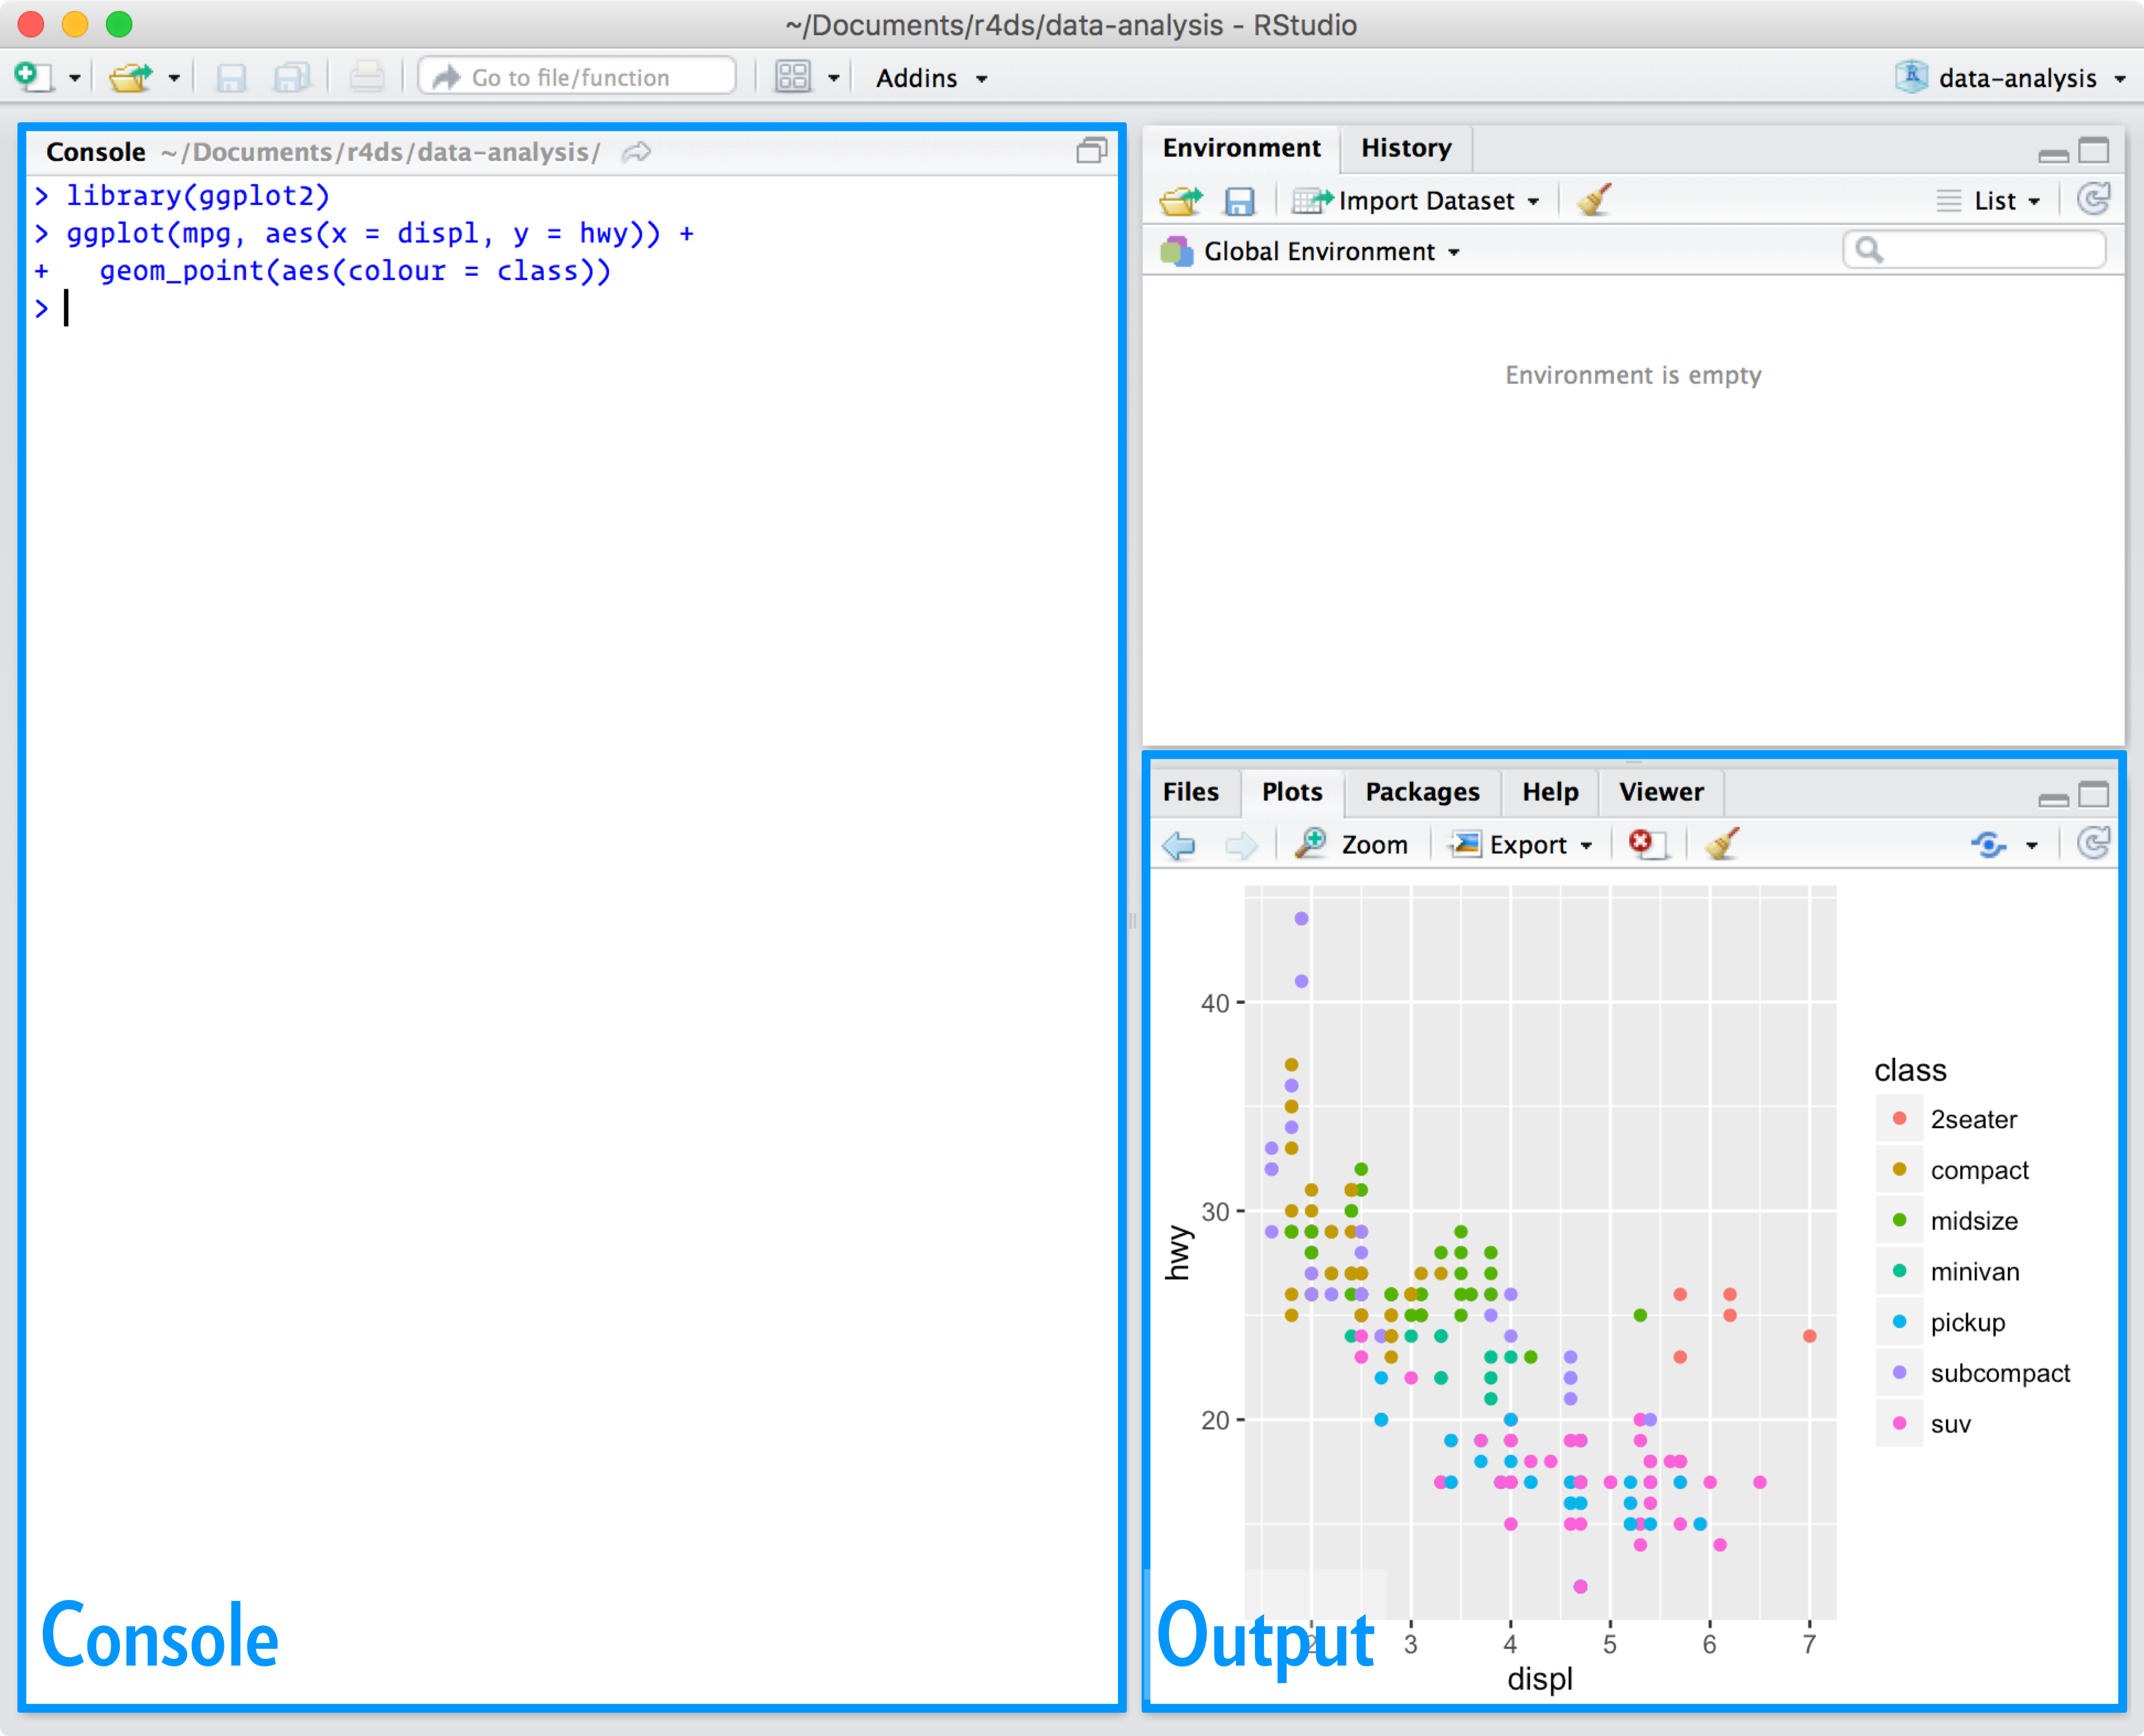
\includegraphics[width=0.9\linewidth]{images/rstudio-console} \end{center}

You can type R code into the \emph{Console} part of the interface and
press the enter key to run the code.

\subsection{R packages}\label{r-packages}

An R package is a collection of R code and documentation that can be
installed to enhance the standard R environment with additional
functionality. Currently, there are over ten thousand R packages
available on CRAN. Each of these R packages (mostly) aim to serve a
specific need, such as
\href{https://cran.r-project.org/web/packages/readxl/index.html}{reading
Excel spreadsheets},
\href{https://cran.r-project.org/web/packages/MODIStsp/index.html}{downloading
satellite imagery data},
\href{https://cran.r-project.org/web/packages/wdpar/index.html}{downloading
and cleaning protected area data}, or
\href{https://cran.r-project.org/web/packages/ENMeval/index.html}{fitting
environmental niche models}. In fact, R has such a diverse ecosystem of
R packages, that the question is (generally) not ``can I use R to do
\ldots{}?'' but ``what R package can I use to \ldots{}?''. During this
workshop, we will use various R packages. To install these R packages,
please run enter the code below in the \emph{Console} part of the
RStudio interface and press enter. Please note that you will require an
internet connection to install the packages and the installation process
may take a while to complete.

\begin{Shaded}
\begin{Highlighting}[]
\KeywordTok{install.packages}\NormalTok{(}\KeywordTok{c}\NormalTok{(}\StringTok{"sf"}\NormalTok{, }\StringTok{"tidyverse"}\NormalTok{, }\StringTok{"sp"}\NormalTok{, }\StringTok{"rgeos"}\NormalTok{, }\StringTok{"rgdal"}\NormalTok{, }\StringTok{"raster"}\NormalTok{,}
                   \StringTok{"prioritizr"}\NormalTok{, }\StringTok{"prioritizrdata"} \StringTok{"Rsymphony"}\NormalTok{, }\StringTok{"mapview"}\NormalTok{))}
\end{Highlighting}
\end{Shaded}

\section{Further reading}\label{further-reading}

There is a wealth of resources available for learning how to use R.
Although not required for this workshop, I would highly recommend that
you read \href{https://r4ds.had.co.nz/}{\emph{R for Data Science} by
Garrett Grolemund and Hadley Wickham}. \textbf{This veritable trove of R
goodness is freely available online.} If you spend a week going through
this book then you will save months debugging and rerunning incorrect
code. I would urge any and all ecologists -- especially those working on
Masters or PhD degrees -- to read this book. I even bought this book as
a Christmas present for my sister---and, yes, she was happy to receive
it! For intermediate users looking to skill-up, I would recommend the
\href{http://shop.oreilly.com/product/9781593273842.do}{\emph{The Art of
R Programming: A Tour of Statistical Software Design} by Norman Matloff}
and \href{https://adv-r.hadley.nz/}{\emph{Advanced R} by Hadley
Wickham}. Finally, if you wish to learn more about using R as a
geospatial information system (GIS), I would recommend
\href{https://geocompr.robinlovelace.net/}{\emph{Geocomputation with R}
by Robin Lovelace, Jakub Nowosad, and Jannes Muenchow} which is also
freely available online. I also recommend
\href{https://www.springer.com/gp/book/9781461476177}{\emph{Applied
Spatial Data Analysis} by Roger S. Bivand, Edzer Pebesma, and Virgilio
Gómez-Rubio} too.

\chapter{Data}\label{data}

\section{Starting out}\label{starting-out}

We will start by opening RStudio. Ideally, you will have already
installed both R and Rstudio before the workshop. If you have not done
this already, then please see the \protect\hyperlink{setup}{Setting up
your computer} section. After opening RStudio, enter the following R
code to attach the R packages we will use in this workshop.

\begin{Shaded}
\begin{Highlighting}[]
\CommentTok{# load packages}
\KeywordTok{library}\NormalTok{(tidyverse)}
\KeywordTok{library}\NormalTok{(prioritizr)}
\KeywordTok{library}\NormalTok{(rgdal)}
\KeywordTok{library}\NormalTok{(raster)}
\KeywordTok{library}\NormalTok{(mapview)}
\end{Highlighting}
\end{Shaded}

You should have already downloaded the data for the prioritizr module of
this workshop. If you have not already done so, you can download it from
here:
\url{https://github.com/prioritizr/cibio-workshop/raw/master/data.zip}.
After downloading the data, you can unzip the data into a new folder.
Next, you will need to set the working directory to this new folder. To
achieve this, click on the \emph{Session} button on the RStudio menu
bar, then click \emph{Set working directory}, and then \emph{Choose
Directory}.

\begin{figure}
\centering
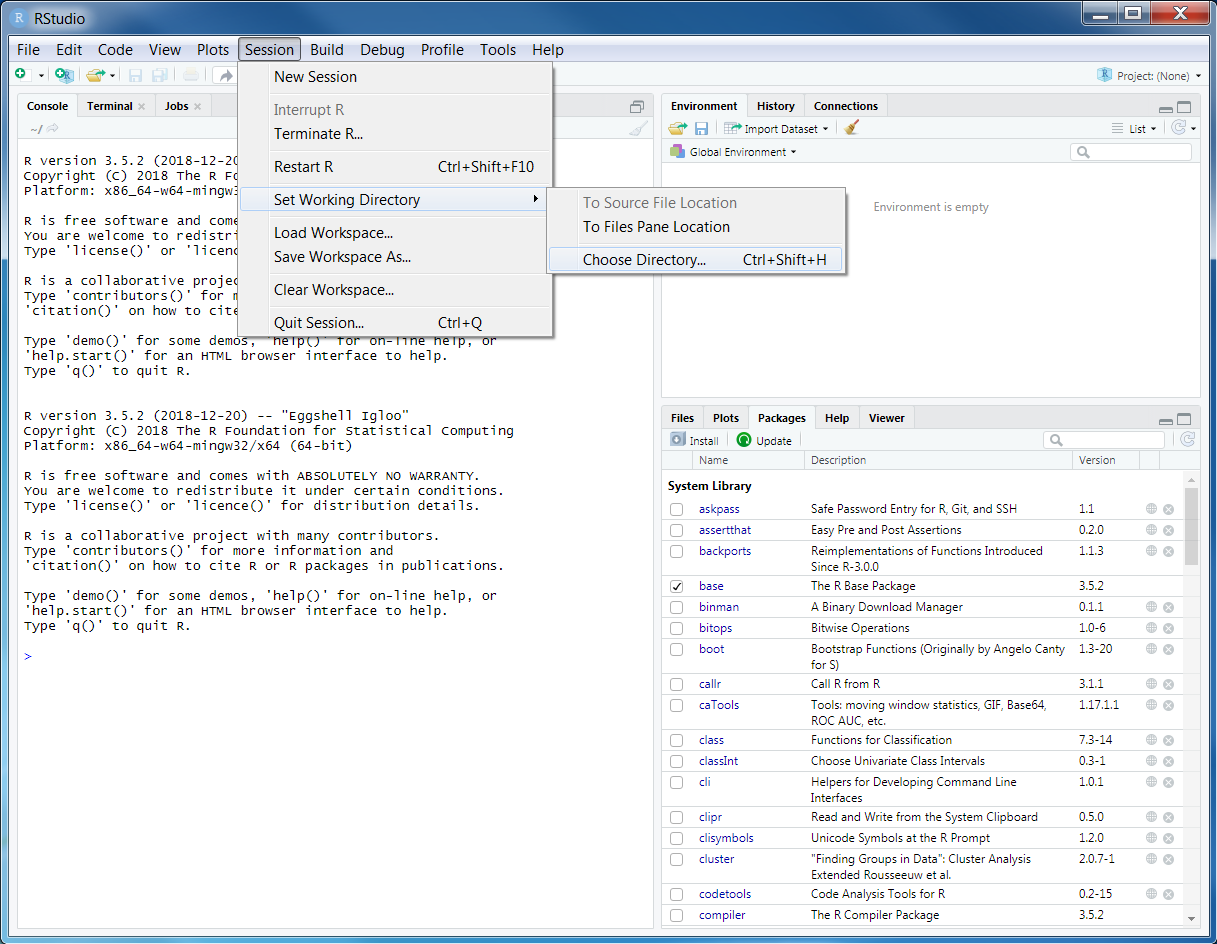
\includegraphics{images/rstudio-wd.png}
\caption{}
\end{figure}

Now navigate to the folder where you unzipped the data and select
\emph{Open}. You can verify that you have correctly set the working
directory using the following R code. You should see the output
\texttt{TRUE}.

\begin{Shaded}
\begin{Highlighting}[]
\KeywordTok{file.exists}\NormalTok{(}\StringTok{"data/pu.shp"}\NormalTok{)}
\end{Highlighting}
\end{Shaded}

\begin{verbatim}
## [1] TRUE
\end{verbatim}

\section{Data import}\label{data-import}

Now that we have downloaded the dataset, we will need to import it into
our R session. Specifically, this data was obtained from the
``Introduction to Marxan'' course and was originally a subset of a
larger spatial prioritization project performed under contract to
Australia's Department of Environment and Water Resources. It contains
vector-based planning unit data (\texttt{pu.shp})and the raster-based
data describing the spatial distributions of 62 vegetation classes
(\texttt{vegetation.tif}) in Tasmania, Australia. We can import the data
into our R session using the following code.

\begin{Shaded}
\begin{Highlighting}[]
\CommentTok{# import planning unit data}
\NormalTok{pu_data <-}\StringTok{ }\KeywordTok{readOGR}\NormalTok{(}\StringTok{"data/pu.shp"}\NormalTok{)}
\end{Highlighting}
\end{Shaded}

\begin{verbatim}
## OGR data source with driver: ESRI Shapefile 
## Source: "/home/travis/build/prioritizr/cibio-workshop/data/pu.shp", layer: "pu"
## with 1130 features
## It has 5 fields
\end{verbatim}

\begin{Shaded}
\begin{Highlighting}[]
\CommentTok{# import vegetation data}
\NormalTok{veg_data <-}\StringTok{ }\KeywordTok{stack}\NormalTok{(}\StringTok{"data/vegetation.tif"}\NormalTok{)}
\end{Highlighting}
\end{Shaded}

\section{Planning unit data}\label{planning-unit-data}

The planning unit data contains spatial data describing the geometry for
each planning unit and attribute data with information about each
planning unit (e.g.~cost values). Let's investigate the
\texttt{pu\_data} object. The attribute data contains 5 columns with
contain the following information: * \texttt{id}: unique identifiers for
each planning unit * \texttt{cost}: acquisition cost values for each
planning unit * \texttt{status}: status information for each planning
unit (only relevant with Marxan) * \texttt{locked\_in}: binary values
(i.e.~one or zero) indicating if planning units are covered by protected
areas or not. * \texttt{locked\_out}: binary values (i.e.~one or zero)
indicating if planning units cannot be managed as a protected area
because they contain too much anthropologically altered land.

\begin{Shaded}
\begin{Highlighting}[]
\CommentTok{# print a short summary of the data}
\KeywordTok{print}\NormalTok{(pu_data)}
\end{Highlighting}
\end{Shaded}

\begin{verbatim}
## class       : SpatialPolygonsDataFrame 
## features    : 1130 
## extent      : 1080623, 1399989, -4840595, -4497092  (xmin, xmax, ymin, ymax)
## crs         : +proj=aea +lat_1=-18 +lat_2=-36 +lat_0=0 +lon_0=132 +x_0=0 +y_0=0 +ellps=GRS80 +units=m +no_defs 
## variables   : 5
## names       :   id,              cost, status, locked_in, locked_out 
## min values  :    1, 0.192488262910798,      0,         0,          0 
## max values  : 1130,  61.9272727272727,      2,         1,          0
\end{verbatim}

\begin{Shaded}
\begin{Highlighting}[]
\CommentTok{# plot the planning unit data}
\KeywordTok{plot}\NormalTok{(pu_data)}
\end{Highlighting}
\end{Shaded}

\begin{center}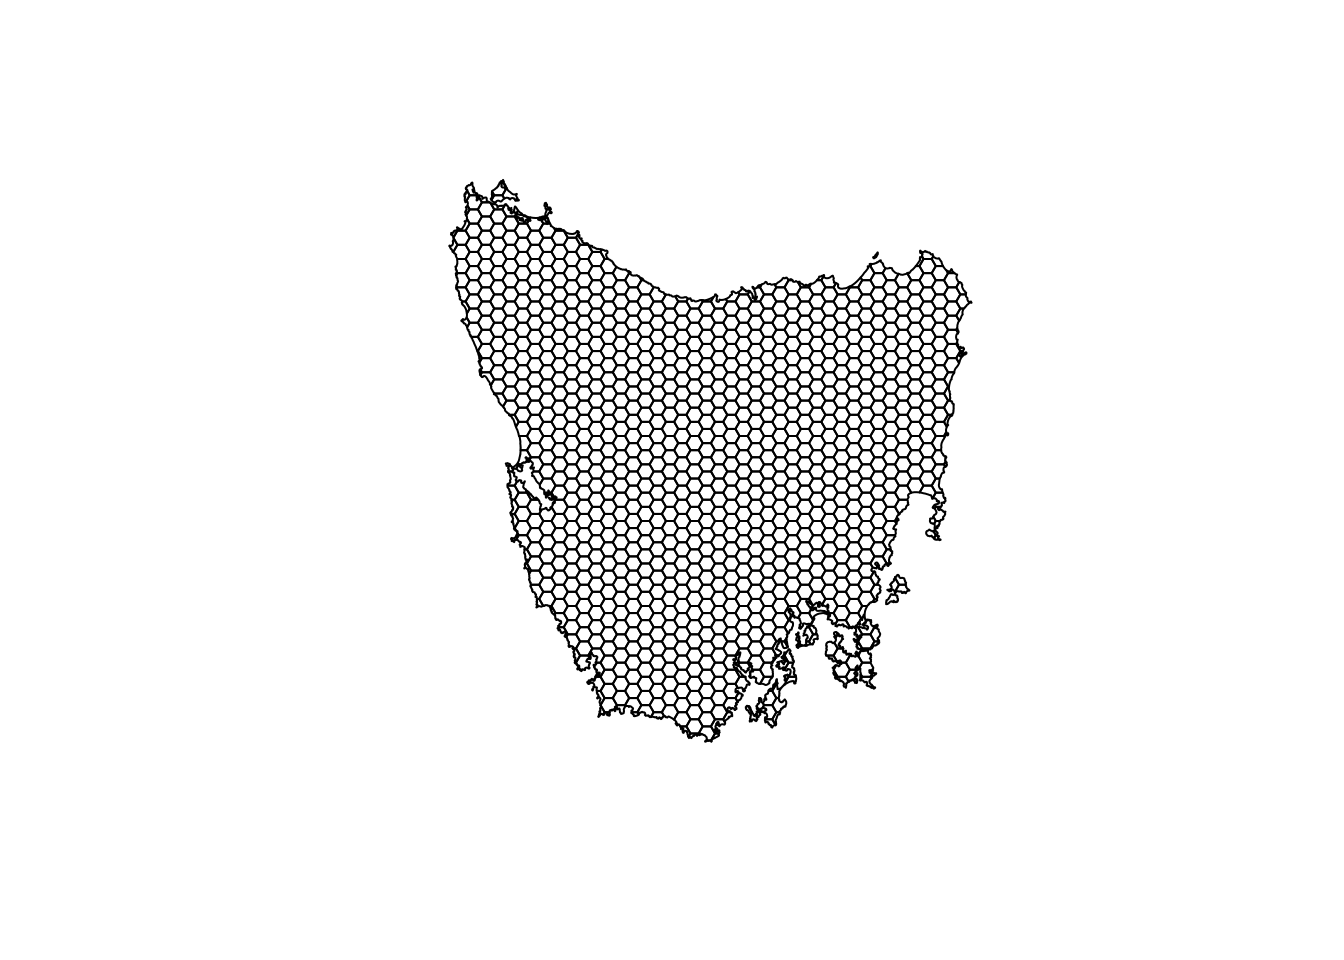
\includegraphics{prioritizr-workshop-manual_files/figure-latex/unnamed-chunk-10-1} \end{center}

\begin{Shaded}
\begin{Highlighting}[]
\CommentTok{# plot an interactive map of the planning unit data}
\KeywordTok{mapview}\NormalTok{(pu_data)}
\end{Highlighting}
\end{Shaded}

\begin{Shaded}
\begin{Highlighting}[]
\CommentTok{# print the structure of object}
\KeywordTok{str}\NormalTok{(pu_data, }\DataTypeTok{max.level =} \DecValTok{2}\NormalTok{)}
\end{Highlighting}
\end{Shaded}

\begin{verbatim}
## Formal class 'SpatialPolygonsDataFrame' [package "sp"] with 5 slots
##   ..@ data       :'data.frame':  1130 obs. of  5 variables:
##   ..@ polygons   :List of 1130
##   ..@ plotOrder  : int [1:1130] 217 973 506 645 705 975 253 271 704 889 ...
##   ..@ bbox       : num [1:2, 1:2] 1080623 -4840595 1399989 -4497092
##   .. ..- attr(*, "dimnames")=List of 2
##   ..@ proj4string:Formal class 'CRS' [package "sp"] with 1 slot
\end{verbatim}

\begin{Shaded}
\begin{Highlighting}[]
\CommentTok{# print the class of the object}
\KeywordTok{class}\NormalTok{(pu_data)}
\end{Highlighting}
\end{Shaded}

\begin{verbatim}
## [1] "SpatialPolygonsDataFrame"
## attr(,"package")
## [1] "sp"
\end{verbatim}

\begin{Shaded}
\begin{Highlighting}[]
\CommentTok{# print the slots of the object}
\KeywordTok{slotNames}\NormalTok{(pu_data)}
\end{Highlighting}
\end{Shaded}

\begin{verbatim}
## [1] "data"        "polygons"    "plotOrder"   "bbox"        "proj4string"
\end{verbatim}

\begin{Shaded}
\begin{Highlighting}[]
\CommentTok{# print the geometry for the 80th planning unit}
\NormalTok{pu_data}\OperatorTok{@}\NormalTok{polygons[[}\DecValTok{80}\NormalTok{]]}
\end{Highlighting}
\end{Shaded}

\begin{verbatim}
## An object of class "Polygons"
## Slot "Polygons":
## [[1]]
## An object of class "Polygon"
## Slot "labpt":
## [1]  1289177 -4558185
## 
## Slot "area":
## [1] 1060361
## 
## Slot "hole":
## [1] FALSE
## 
## Slot "ringDir":
## [1] 1
## 
## Slot "coords":
##          [,1]     [,2]
##  [1,] 1288123 -4558431
##  [2,] 1287877 -4558005
##  [3,] 1288177 -4558019
##  [4,] 1288278 -4558054
##  [5,] 1288834 -4558038
##  [6,] 1289026 -4557929
##  [7,] 1289168 -4557928
##  [8,] 1289350 -4557790
##  [9,] 1289517 -4557744
## [10,] 1289618 -4557773
## [11,] 1289836 -4557965
## [12,] 1290000 -4557984
## [13,] 1290025 -4557987
## [14,] 1290144 -4558168
## [15,] 1290460 -4558431
## [16,] 1288123 -4558431
## 
## 
## 
## Slot "plotOrder":
## [1] 1
## 
## Slot "labpt":
## [1]  1289177 -4558185
## 
## Slot "ID":
## [1] "79"
## 
## Slot "area":
## [1] 1060361
\end{verbatim}

\begin{Shaded}
\begin{Highlighting}[]
\CommentTok{# print the coordinate reference system}
\KeywordTok{print}\NormalTok{(pu_data}\OperatorTok{@}\NormalTok{proj4string)}
\end{Highlighting}
\end{Shaded}

\begin{verbatim}
## CRS arguments:
##  +proj=aea +lat_1=-18 +lat_2=-36 +lat_0=0 +lon_0=132 +x_0=0 +y_0=0
## +ellps=GRS80 +units=m +no_defs
\end{verbatim}

\begin{Shaded}
\begin{Highlighting}[]
\CommentTok{# print number of planning units (geometries) in the data}
\KeywordTok{nrow}\NormalTok{(pu_data)}
\end{Highlighting}
\end{Shaded}

\begin{verbatim}
## [1] 1130
\end{verbatim}

\begin{Shaded}
\begin{Highlighting}[]
\CommentTok{# print the first six rows in the attribute data}
\KeywordTok{head}\NormalTok{(pu_data}\OperatorTok{@}\NormalTok{data)}
\end{Highlighting}
\end{Shaded}

\begin{verbatim}
##   id     cost status locked_in locked_out
## 0  1 60.24638      0         0          0
## 1  2 19.86301      0         0          0
## 2  3 59.68051      0         0          0
## 3  4 32.41614      0         0          0
## 4  5 26.17706      0         0          0
## 5  6 51.26218      0         0          0
\end{verbatim}

\begin{Shaded}
\begin{Highlighting}[]
\CommentTok{# print the first six values in the cost column of the attribute data}
\KeywordTok{head}\NormalTok{(pu_data}\OperatorTok{$}\NormalTok{cost)}
\end{Highlighting}
\end{Shaded}

\begin{verbatim}
## [1] 60.24638 19.86301 59.68051 32.41614 26.17706 51.26218
\end{verbatim}

\begin{Shaded}
\begin{Highlighting}[]
\CommentTok{# print the highest cost value}
\KeywordTok{max}\NormalTok{(pu_data}\OperatorTok{$}\NormalTok{cost)}
\end{Highlighting}
\end{Shaded}

\begin{verbatim}
## [1] 61.92727
\end{verbatim}

\begin{Shaded}
\begin{Highlighting}[]
\CommentTok{# print the smallest cost value}
\KeywordTok{min}\NormalTok{(pu_data}\OperatorTok{$}\NormalTok{cost)}
\end{Highlighting}
\end{Shaded}

\begin{verbatim}
## [1] 0.1924883
\end{verbatim}

\begin{Shaded}
\begin{Highlighting}[]
\CommentTok{# print average cost value}
\KeywordTok{mean}\NormalTok{(pu_data}\OperatorTok{$}\NormalTok{cost)}
\end{Highlighting}
\end{Shaded}

\begin{verbatim}
## [1] 25.13536
\end{verbatim}

\begin{Shaded}
\begin{Highlighting}[]
\CommentTok{# plot a map of the planning unit cost data}
\KeywordTok{spplot}\NormalTok{(pu_data, }\StringTok{"cost"}\NormalTok{)}
\end{Highlighting}
\end{Shaded}

\begin{center}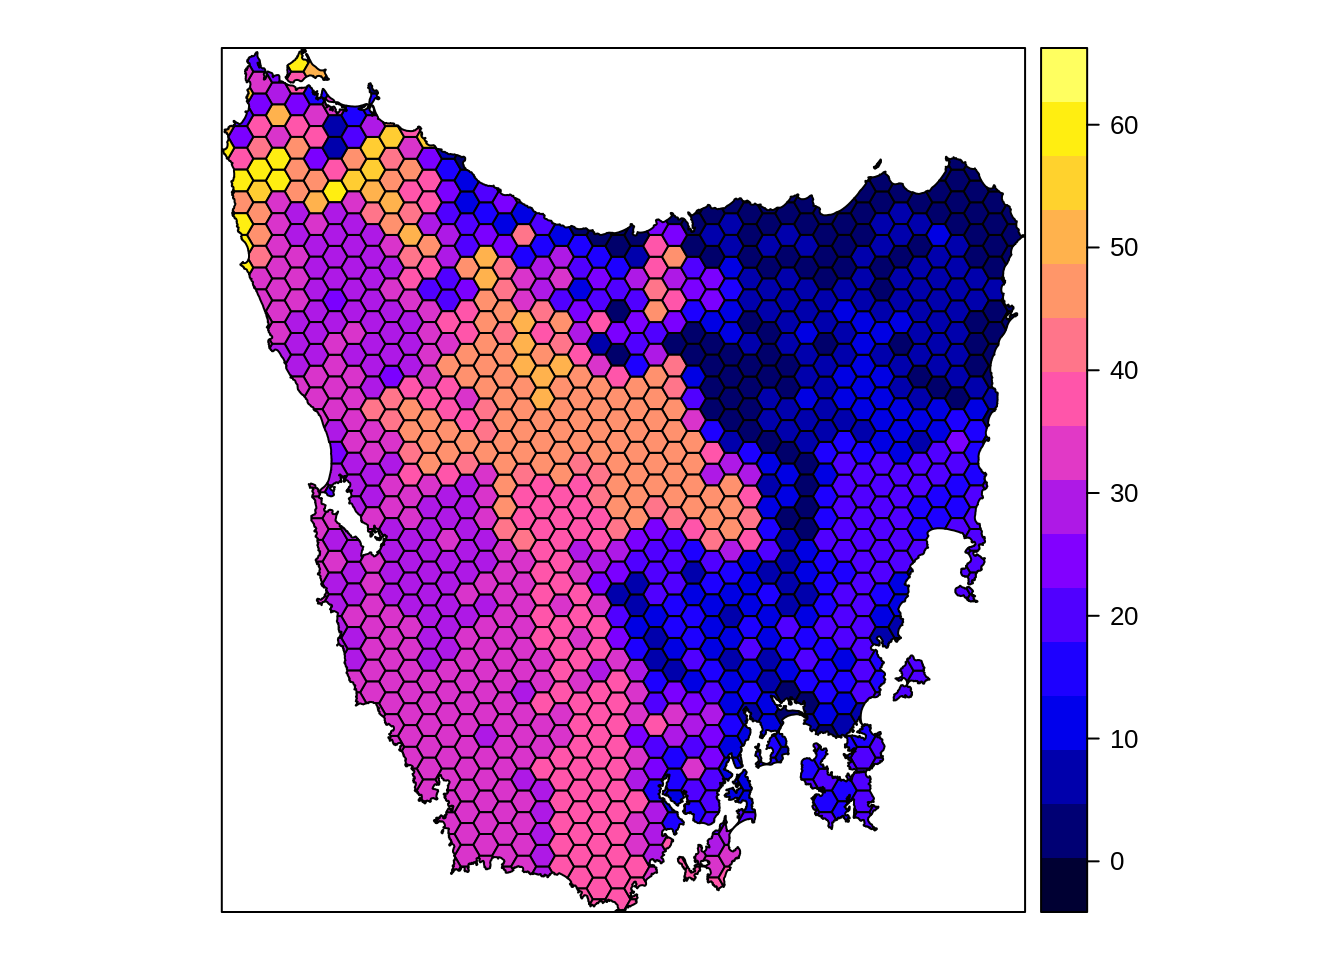
\includegraphics{prioritizr-workshop-manual_files/figure-latex/unnamed-chunk-12-1} \end{center}

\begin{Shaded}
\begin{Highlighting}[]
\CommentTok{# plot an interactive map of the planning unit cost data}
\KeywordTok{mapview}\NormalTok{(pu_data, }\DataTypeTok{zcol =} \StringTok{"cost"}\NormalTok{)}
\end{Highlighting}
\end{Shaded}

\clearpage

Now, you can try and answer some questions about the planning unit data.

\BeginKnitrBlock{rmdquestion}
\begin{enumerate}
\def\labelenumi{\arabic{enumi}.}
\tightlist
\item
  How many planning units are in the planning unit data?
\item
  What is the highest cost value?
\item
  How many planning units are covered by the protected areas (hint:
  \texttt{sum(x)})?
\item
  What is the proportion of the planning units that are covered by the
  protected areas (hint: \texttt{mean(x)})?
\item
  How many planning units are dominated by anthropologically altered
  land (hint: \texttt{sum(x)})?
\item
  What is the proportion of planning units dominated by
  anthropologically altered land (hint: \texttt{mean(x)})?
\item
  Can you verify that all values in the \texttt{locked\_in} and
  \texttt{locked\_out} columns are zero or one (hint: \texttt{min(x)}
  and \texttt{max(x)})?.
\item
  Can you verify that none of the planning units are missing cost values
  (hint: \texttt{all(is.finite(x))})?.
\item
  Can you very that none of the planning units have duplicated
  identifiers? (hint: \texttt{sum(duplicated(x))})?
\item
  Is there a spatial pattern in the planning unit cost values (hint:
  make a map).
\item
  Is there a spatial pattern in where most planning units are covered by
  protected areas (hint: make a map of \texttt{locked\_in}).
\end{enumerate}
\EndKnitrBlock{rmdquestion}

\section{Vegetation data}\label{vegetation-data}

The vegetation data describes the spatial distribution of 62 vegetation
classes in the study area. This data is in a raster format and so the
data are organized using a regular spatial grid with square grid cells.
In our case, our raster data contains multiple layers (also called
``bands'') and each layer has corresponds to a spatial grid with exactly
the same area and has exactly the same dimensionality (i.e.~number of
rows, columns, and cells). In this dataset, there are 62 different
regular spatial grids layered on top of each other -- with each layer
corresponding to a different vegetation class -- and each of these
layers contains a grid with 343 columns, 320 rows, and 109760 cells.
Within each layer, each cell corresponds to a 1 by 1 km square. The
values associated with each grid cell contain values (i.e.~one or zero)
indicating the presence or absence of a given vegetation class in the
cell.

\begin{figure}
\centering
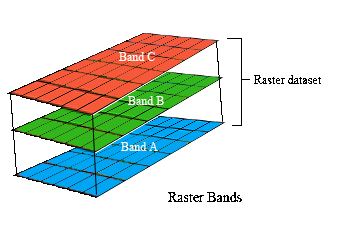
\includegraphics{images/rasterbands.png}
\caption{}
\end{figure}

Let's explore the vegetation data.

\begin{Shaded}
\begin{Highlighting}[]
\CommentTok{# print a short summary of the data}
\KeywordTok{print}\NormalTok{(veg_data)}
\end{Highlighting}
\end{Shaded}

\begin{verbatim}
## class      : RasterStack 
## dimensions : 343, 320, 109760, 62  (nrow, ncol, ncell, nlayers)
## resolution : 1000, 1000  (x, y)
## extent     : 1080496, 1400496, -4841217, -4498217  (xmin, xmax, ymin, ymax)
## crs        : +proj=aea +lat_1=-18 +lat_2=-36 +lat_0=0 +lon_0=132 +x_0=0 +y_0=0 +ellps=GRS80 +units=m +no_defs 
## names      : vegetation.1, vegetation.2, vegetation.3, vegetation.4, vegetation.5, vegetation.6, vegetation.7, vegetation.8, vegetation.9, vegetation.10, vegetation.11, vegetation.12, vegetation.13, vegetation.14, vegetation.15, ... 
## min values :            0,            0,            0,            0,            0,            0,            0,            0,            0,             0,             0,             0,             0,             0,             0, ... 
## max values :            1,            1,            1,            1,            1,            1,            1,            1,            1,             1,             1,             1,             1,             1,             1, ...
\end{verbatim}

\begin{Shaded}
\begin{Highlighting}[]
\CommentTok{# plot a map of the 36th vegetation class}
\KeywordTok{plot}\NormalTok{(veg_data[[}\DecValTok{36}\NormalTok{]])}
\end{Highlighting}
\end{Shaded}

\begin{center}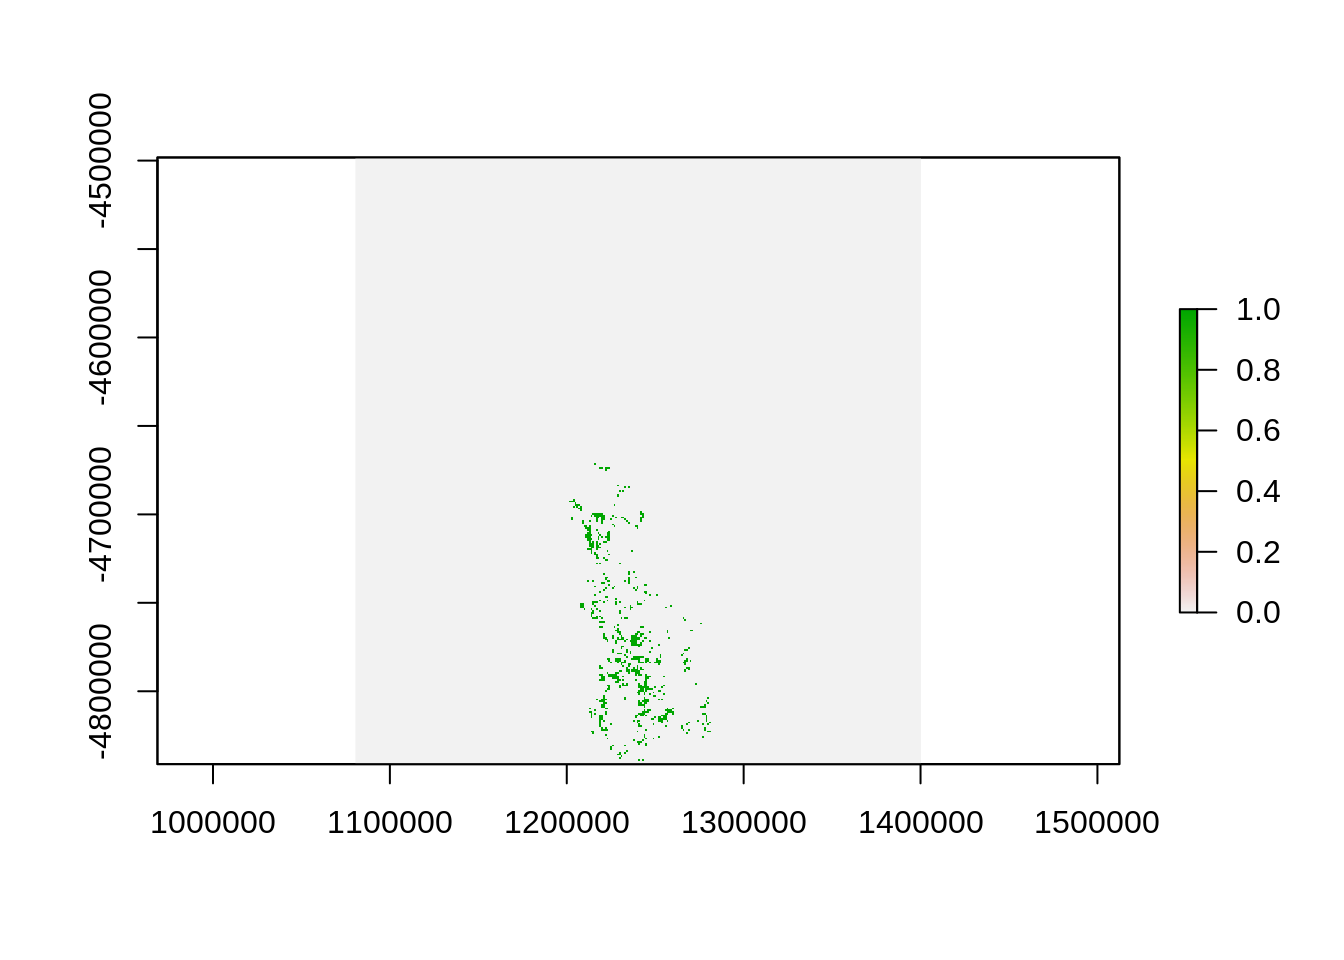
\includegraphics{prioritizr-workshop-manual_files/figure-latex/unnamed-chunk-16-1} \end{center}

\begin{Shaded}
\begin{Highlighting}[]
\CommentTok{# plot an interactive map of the 36th vegetation class}
\KeywordTok{mapview}\NormalTok{(veg_data[[}\DecValTok{36}\NormalTok{]])}
\end{Highlighting}
\end{Shaded}

\begin{Shaded}
\begin{Highlighting}[]
\CommentTok{# print number of rows in the data}
\KeywordTok{nrow}\NormalTok{(veg_data)}
\end{Highlighting}
\end{Shaded}

\begin{verbatim}
## [1] 343
\end{verbatim}

\begin{Shaded}
\begin{Highlighting}[]
\CommentTok{# print number of columns  in the data}
\KeywordTok{ncol}\NormalTok{(veg_data)}
\end{Highlighting}
\end{Shaded}

\begin{verbatim}
## [1] 320
\end{verbatim}

\begin{Shaded}
\begin{Highlighting}[]
\CommentTok{# print number of cells in the data}
\KeywordTok{ncell}\NormalTok{(veg_data)}
\end{Highlighting}
\end{Shaded}

\begin{verbatim}
## [1] 109760
\end{verbatim}

\begin{Shaded}
\begin{Highlighting}[]
\CommentTok{# print number of layers in the data}
\KeywordTok{nlayers}\NormalTok{(veg_data)}
\end{Highlighting}
\end{Shaded}

\begin{verbatim}
## [1] 62
\end{verbatim}

\begin{Shaded}
\begin{Highlighting}[]
\CommentTok{# print  resolution on the x-axis}
\KeywordTok{xres}\NormalTok{(veg_data)}
\end{Highlighting}
\end{Shaded}

\begin{verbatim}
## [1] 1000
\end{verbatim}

\begin{Shaded}
\begin{Highlighting}[]
\CommentTok{# print resolution on the y-axis}
\KeywordTok{yres}\NormalTok{(veg_data)}
\end{Highlighting}
\end{Shaded}

\begin{verbatim}
## [1] 1000
\end{verbatim}

\begin{Shaded}
\begin{Highlighting}[]
\CommentTok{# print spatial extent of the grid, i.e. coordinates for corners}
\KeywordTok{extent}\NormalTok{(veg_data)}
\end{Highlighting}
\end{Shaded}

\begin{verbatim}
## class      : Extent 
## xmin       : 1080496 
## xmax       : 1400496 
## ymin       : -4841217 
## ymax       : -4498217
\end{verbatim}

\begin{Shaded}
\begin{Highlighting}[]
\CommentTok{# print the coordinate reference system}
\KeywordTok{print}\NormalTok{(veg_data}\OperatorTok{@}\NormalTok{crs)}
\end{Highlighting}
\end{Shaded}

\begin{verbatim}
## CRS arguments:
##  +proj=aea +lat_1=-18 +lat_2=-36 +lat_0=0 +lon_0=132 +x_0=0 +y_0=0
## +ellps=GRS80 +units=m +no_defs
\end{verbatim}

\begin{Shaded}
\begin{Highlighting}[]
\CommentTok{# print a summary of the first layer in the stack}
\KeywordTok{print}\NormalTok{(veg_data[[}\DecValTok{1}\NormalTok{]])}
\end{Highlighting}
\end{Shaded}

\begin{verbatim}
## class      : RasterLayer 
## band       : 1  (of  62  bands)
## dimensions : 343, 320, 109760  (nrow, ncol, ncell)
## resolution : 1000, 1000  (x, y)
## extent     : 1080496, 1400496, -4841217, -4498217  (xmin, xmax, ymin, ymax)
## crs        : +proj=aea +lat_1=-18 +lat_2=-36 +lat_0=0 +lon_0=132 +x_0=0 +y_0=0 +ellps=GRS80 +units=m +no_defs 
## source     : /home/travis/build/prioritizr/cibio-workshop/data/vegetation.tif 
## names      : vegetation.1 
## values     : 0, 1  (min, max)
\end{verbatim}

\begin{Shaded}
\begin{Highlighting}[]
\CommentTok{# print the value in the 800th cell in the first layer of the stack}
\KeywordTok{print}\NormalTok{(veg_data[[}\DecValTok{1}\NormalTok{]][}\DecValTok{800}\NormalTok{])}
\end{Highlighting}
\end{Shaded}

\begin{verbatim}
##   
## 0
\end{verbatim}

\begin{Shaded}
\begin{Highlighting}[]
\CommentTok{# print the value of the cell located in the 30th row and the 60th column of}
\CommentTok{# the first layer}
\KeywordTok{print}\NormalTok{(veg_data[[}\DecValTok{1}\NormalTok{]][}\DecValTok{30}\NormalTok{, }\DecValTok{60}\NormalTok{])}
\end{Highlighting}
\end{Shaded}

\begin{verbatim}
##   
## 0
\end{verbatim}

\begin{Shaded}
\begin{Highlighting}[]
\CommentTok{# calculate the sum of all the cell values in the first layer}
\KeywordTok{cellStats}\NormalTok{(veg_data[[}\DecValTok{1}\NormalTok{]], }\StringTok{"sum"}\NormalTok{)}
\end{Highlighting}
\end{Shaded}

\begin{verbatim}
## [1] 36
\end{verbatim}

\begin{Shaded}
\begin{Highlighting}[]
\CommentTok{# calculate the maximum value of all the cell values in the first layer}
\KeywordTok{cellStats}\NormalTok{(veg_data[[}\DecValTok{1}\NormalTok{]], }\StringTok{"max"}\NormalTok{)}
\end{Highlighting}
\end{Shaded}

\begin{verbatim}
## [1] 1
\end{verbatim}

\begin{Shaded}
\begin{Highlighting}[]
\CommentTok{# calculate the minimum value of all the cell values in the first layer}
\KeywordTok{cellStats}\NormalTok{(veg_data[[}\DecValTok{1}\NormalTok{]], }\StringTok{"min"}\NormalTok{)}
\end{Highlighting}
\end{Shaded}

\begin{verbatim}
## [1] 0
\end{verbatim}

\begin{Shaded}
\begin{Highlighting}[]
\CommentTok{# calculate the mean value of all the cell values in the first layer}
\KeywordTok{cellStats}\NormalTok{(veg_data[[}\DecValTok{1}\NormalTok{]], }\StringTok{"mean"}\NormalTok{)}
\end{Highlighting}
\end{Shaded}

\begin{verbatim}
## [1] 0.0003279883
\end{verbatim}

\begin{Shaded}
\begin{Highlighting}[]
\CommentTok{# calculate the maximum value in each layer}
\KeywordTok{data.frame}\NormalTok{(}\DataTypeTok{max =} \KeywordTok{cellStats}\NormalTok{(veg_data, }\StringTok{"max"}\NormalTok{))}
\end{Highlighting}
\end{Shaded}

\begin{verbatim}
##    max
## 1    1
## 2    1
## 3    1
## 4    1
## 5    1
## 6    1
## 7    1
## 8    1
## 9    1
## 10   1
## 11   1
## 12   1
## 13   1
## 14   1
## 15   1
## 16   1
## 17   1
## 18   1
## 19   1
## 20   1
## 21   1
## 22   1
## 23   1
## 24   1
## 25   1
## 26   1
## 27   1
## 28   1
## 29   1
## 30   1
## 31   1
## 32   1
## 33   1
## 34   1
## 35   1
## 36   1
## 37   1
## 38   1
## 39   1
## 40   1
## 41   1
## 42   1
## 43   1
## 44   1
## 45   1
## 46   1
## 47   1
## 48   1
## 49   1
## 50   1
## 51   1
## 52   1
## 53   1
## 54   1
## 55   1
## 56   1
## 57   1
## 58   1
## 59   1
## 60   1
## 61   1
## 62   1
\end{verbatim}

Now, you can try and answer some questions about the vegetation data.

\BeginKnitrBlock{rmdquestion}
\begin{enumerate}
\def\labelenumi{\arabic{enumi}.}
\tightlist
\item
  What part of the study area is the 51st vegetation class found in
  (hint: make a map)?
\item
  How many rows does the 23rd layer contain?
\item
  Is the third vegetation class present at the 400th cell?
\item
  How many cells contain the 56th vegetation class?
\item
  What proportion of cells contain the 12th vegetation class?
\item
  Which vegetation class is present in the greatest number of cells?
\item
  Make an new object by summing together all the layer values into a
  single grid (i.e.
  \texttt{sum\_veg\_data\ \textless{}-\ sum(veg\_data)}) and make a map
  showing this data (i.e. \texttt{plot(sum\_veg\_data)}). What does it
  mean if cells contain zeros in this new object? What reasons could
  there be to explain why some cells in this new object contain zeros?
\end{enumerate}
\EndKnitrBlock{rmdquestion}

\chapter{Gap analysis}\label{gap-analysis}

TODO.

\chapter{Spatial prioritizations}\label{spatial-prioritizations}

TODO.

\chapter{Irreplaceability}\label{irreplaceability}

TODO.

\chapter{Acknowledgements}\label{acknowledgements}

Many thanks to \href{https://icons8.com}{Icons8} for providing the icons
used in this manual.

\bibliography{references.bib}


\end{document}
